
%%%%%%%%%%%%%%%%%%%%%
\section{Champ électrique}
%%%%%%%%%%%%%%%%%%%%%
%
Le champ électrique est défini comme un {\it intermédiaire de calcul} entre la présence d'une charge électrique $Q_1$ et la force exercé par celle-ci sur une charge électrique $Q_2$.
%L'expérience du pendule électrostatique peut se modéliser par des {\it forces électrostatiques} s'exerçant entre les particules chargées. Ce modèle suppose une {\it action à distance}.
%La notion de champs permet de modéliser cette action entre les charges électriques : une . Le champ exerce une force sur les charges électriques.

% Dans un second temps, elle peut se modéliser par  en disant qu'une particule chargée crée un champ électrostatique en tout point de l'espace et qu'une particule chargée placé dans un champ électrostatique subit une force.

\subsection{Vision "force de coulomb"}


\vspace{0.5cm}

\begin{center}
\setlength{\unitlength}{1cm}
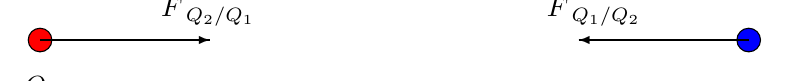
\begin{tikzpicture}
\draw [fill=red] (0.5,1.0) circle(0.15);
\put(0.3,0.3){$Q_1$}
\put(0.5,1.0){\vector(1,0){2.16}}
\put(2,1.3){$\overrightarrow{F}_{Q_2/Q_1}$}
\draw [fill=blue] (9.5,1.0) circle(0.15);
\put(9.3,0.2){$Q_2$}
\put(9.5,1.0) {\vector(-1,0){2.16}}
\put(6.9,1.3){$\overrightarrow{F}_{Q_1/Q_2}$}
\end{tikzpicture}
\end{center}

\subsection{Vision "champ électrique"}

La charge électrique (positive) $Q_1$ crée un champ électrique (champ vectoriel représenté ci-dessous en quelque points).

\begin{center}
\tikzstyle{fleche}=[->,line width=1pt]
\begin{tikzpicture}
  \begin{scope}[xshift=0 cm,yshift=0 cm, scale = 1.6]%
\foreach \t in {60,120, ...,360}
\draw [fleche] (\t:1) -- (\t:2.8);
\foreach \t in {30,90, ...,360}
\draw [fleche] (\t:2) -- (\t:2.45);
\foreach \t in {15,45,-15,-45}
\draw [fleche] (\t:3) -- (\t:3.2);
\foreach \t in {15,45,-15,-45}
\draw [fleche] (\t+180:3) -- (\t+180:3.2);
\draw [fill=red] (0,0) circle(0.1) node [above right] {$Q_1$};
  \end{scope}
\end{tikzpicture}
\end{center}

Le champ électrique $\overrightarrow{E}$ exerce une force $\overrightarrow{F}_{\overrightarrow{E}/Q_2}$ sur la charge électrique $Q_2$

\begin{center}
\tikzstyle{fleche}=[->,line width=1pt]
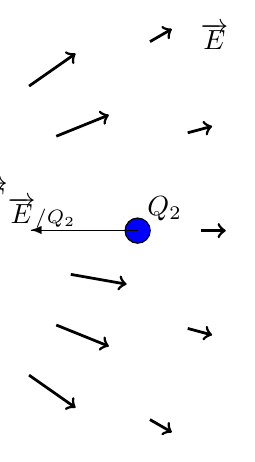
\begin{tikzpicture}
  \begin{scope}[xshift=0 cm,yshift=0 cm, scale = 1.6]%
\foreach \t in {35,-35,-22,-10,22}
\draw [fleche] (\t:2) -- (\t:2.45);
\foreach \t in {0,15,30,-15,-30}
\draw [fleche] (\t:3) -- (\t:3.2);
\draw [fill=blue] (2.5,0) circle(0.1) node [above right] {$Q_2$};
\put(4,0){\vector(-1,0){1.36}}
\put(2,0.3){$\overrightarrow{F}_{\overrightarrow{E}/Q_2}$}
\put(4.8,2.3){$\overrightarrow{E}$}
  \end{scope}
\end{tikzpicture}
\end{center}

Le champ créé par une charge électrique est à priori un outil purement mathématique, un artifice de calcul bien pratique. L'existence de ce "champ électrique" est à priori hypothétique. Néanmoins, son existence permet d'interpréter la transmission de "l'information de présence" entre les charges, de lever l'hypothèse d'une transmission d'information instantanée et immatérielle entre les charges.

%%%%%%%%%%%%%%%%%%%%%%%%%%%%%%%%%%%%%%%%%%%%%%%%%%%%%%%%%%%%%%%%%%%%%%%%%%%%
